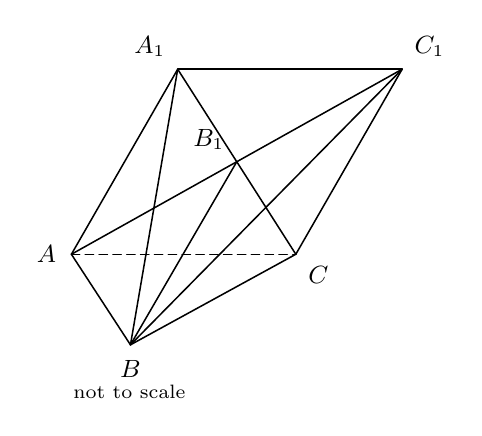
\begin{tikzpicture}[
  x=1cm,
  y=1cm,
  line cap=round,
  line join=round,
  every node/.style={font=\small},
  edge/.style={draw=black, line width=0.55pt}
]
  \coordinate (A) at (0,0);
  \coordinate (B) at (0.75,-1.15);
  \coordinate (C) at (2.85,0);
  \coordinate (A_1) at (1.35,2.35);
  \coordinate (B_1) at (2.10,1.175);
  \coordinate (C_1) at (4.20,2.35);

  % Hidden edge from the source figure.
  \draw[densely dashed, line width=0.55pt] (A) -- (C);

  % Triangular prism edges.
  \draw[edge] (A) -- (B);
  \draw[edge] (B) -- (C);
  \draw[edge] (A) -- (A_1);
  \draw[edge] (B) -- (B_1);
  \draw[edge] (C) -- (C_1);
  \draw[edge] (A_1) -- (B_1);
  \draw[edge] (B_1) -- (C_1);
  \draw[edge] (A_1) -- (C_1);

  % Additional lines appearing in the source geometry diagram.
  \draw[edge] (A_1) -- (B);
  \draw[edge] (A) -- (B_1);
  \draw[edge] (B) -- (C_1);
  \draw[edge] (B_1) -- (C);

  \node[left=2pt] at (A) {$A$};
  \node[below=2pt] at (B) {$B$};
  \node[below right=1pt] at (C) {$C$};
  \node[above left=1pt] at (A_1) {$A_1$};
  \node[above left=1pt] at (B_1) {$B_1$};
  \node[above right=1pt] at (C_1) {$C_1$};
  \node[font=\scriptsize, anchor=west] at (-0.1,-1.75) {not to scale};
\end{tikzpicture}
